In this part, we show that the Fiedler value of every bounded-degree planar graph is $O(1/n)$. We obtain this bound of eigenvalue by showing that every planar graph has a  good geometric embedding.  

\begin{lemma}[Embedding lemma]\label{embedding_lemma} Let $G=(V,E)$ be a graph. Then the Fiedler value of $G$, $\lambda_2$, is given by 

$$
\lambda_2 = \min \frac{\sum_{(i,j)\in E}\|\vv_i-\vv_j\|^2}{\sum_{i=1}^n\|\vv_i^2\|}
$$
where the minimum is taken over vectors $\{\vv_1,...,\vv_n\}\subset R^n$ such that 

$$
\sum_{i=1}^{n}\vv_i=\vzero
$$
where $\vzero$ denotes the zero vector.

\end{lemma}
\begin{proof}
    Because for any Laplacian matrix $L\vone=\vzero$, we know that all-ones vector is the eigenvector corresponding to the eigenvalue 0, $\lambda_2$ could be characterized as 

$$
\lambda_2 = \min \frac{\sum_{(i,j)\in E}(x_i-x_j)^2}{\sum_{i=1}^n(x_i^2)}
$$
where the minimum is taken over real $x_i$'s such that $\sum_{i=1}^{n}x_i=0$. 
(e.g.)
We then rewrite $\vv_i$ as $(v_{i,1}, ..., v_{i,n})$. For all $\{\vv_1, ..., \vv_n\}$, such that $\sum_{i=1}^{n}\vv_i=\vzero$, we have
\begin{align*}
\frac{\sum_{(i,j)\in E}\|\vv_i-\vv_j\|^2}{\sum_{i=1}^n\|\vv_i^2\|} 
& = \frac{\sum_{(i,j)\in E}\sum_{k=1}^{n}(v_{i,k}-v_{j,k})^2}{\sum_{i=1}^n\sum_{k=1}^{n}v_{i,k}^2} \\
& = \frac{\sum_{k=1}^{n}\sum_{(i,j)\in E}(v_{i,k}-v_{j,k})^2}{\sum_{k=1}^{n}\sum_{i=1}^nv_{i,k}^2} \\
\end{align*}
Since for each $k$, we have 
$$
\lambda_2 \leq \frac{\sum_{(i,j)\in E}(v_{i,k}-v_{j,k})^2}{\sum_{i=1}^nv_{i,k}^2} 
$$
therefore
$$
\lambda_2 \leq \frac{\sum_{k=1}^{n}\sum_{(i,j)\in E}(v_{i,k}-v_{j,k})^2}{\sum_{k=1}^{n}\sum_{i=1}^nv_{i,k}^2} 
$$
this follows the fact that $\sum_i x_i / \sum_i y_i \geq \min_i x_i / y_i$ for $x_i, y_i > 0$.

\end{proof}


\begin{theorem}[Koebe-Andreev-Thurston]\label{Koebe-Andreev-Thurston}. Let $G$ be a planar graph with vertex set $V=\{1,...,n\}$, and edge set $E$, there exists a set of disks $\{D_1, ...,D_n\}$ in the plane with disjoint interiors such that $D_i$ touches $D_j$ if and only if $(i,j)\in E$.
\end{theorem}
Such embedding is called a kissing disk embedding of $G$.

\begin{figure}[h]
\centering
\begin{subfigure}[b]{0.45\textwidth}
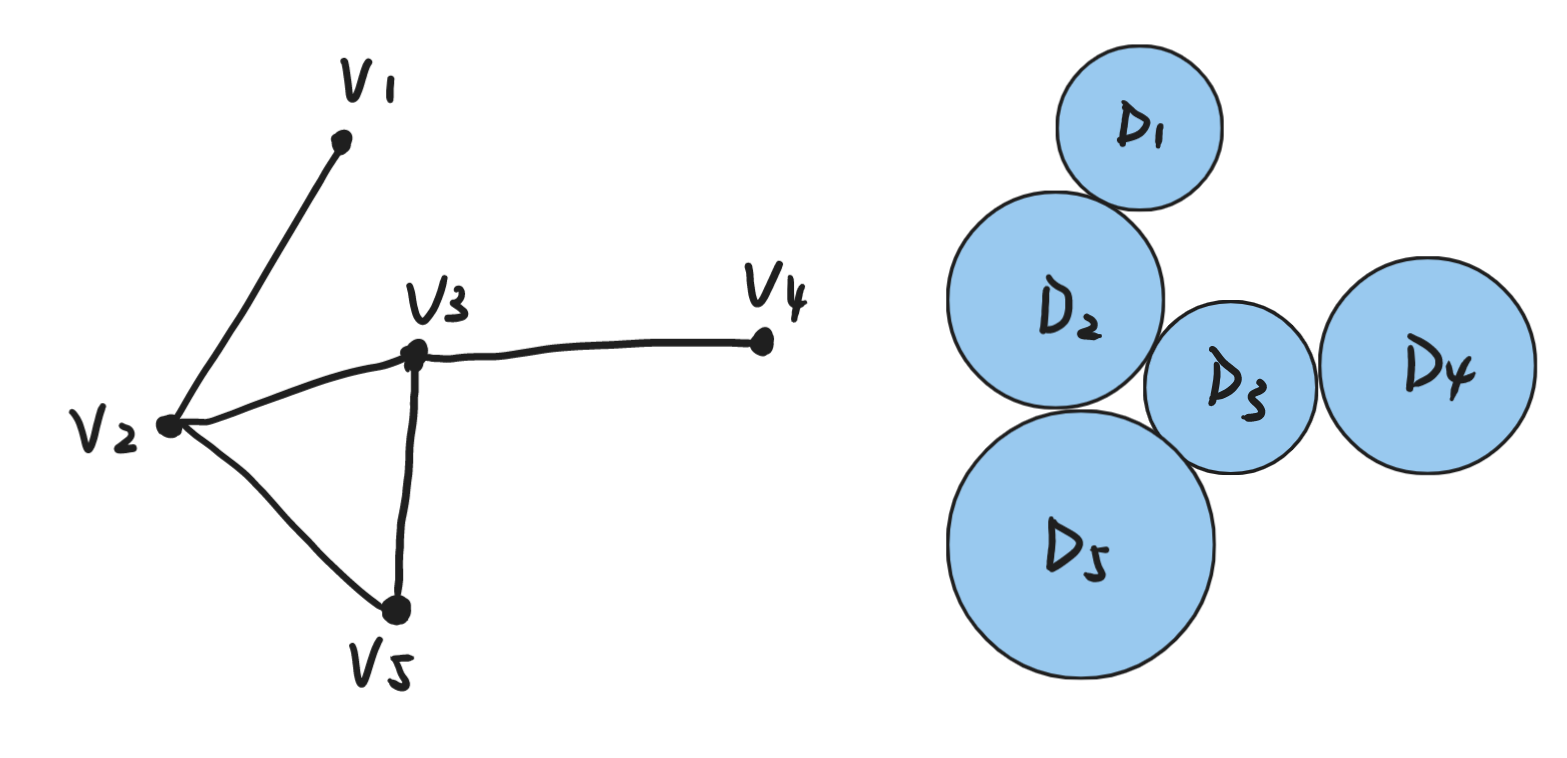
\includegraphics[width=\textwidth]{figures/kissingdisk.png}
\caption{From planar graphs to kissing disks}
\label{fig:kissing-disks}
\end{subfigure}
\hfill
\begin{subfigure}[b]{0.45\textwidth}
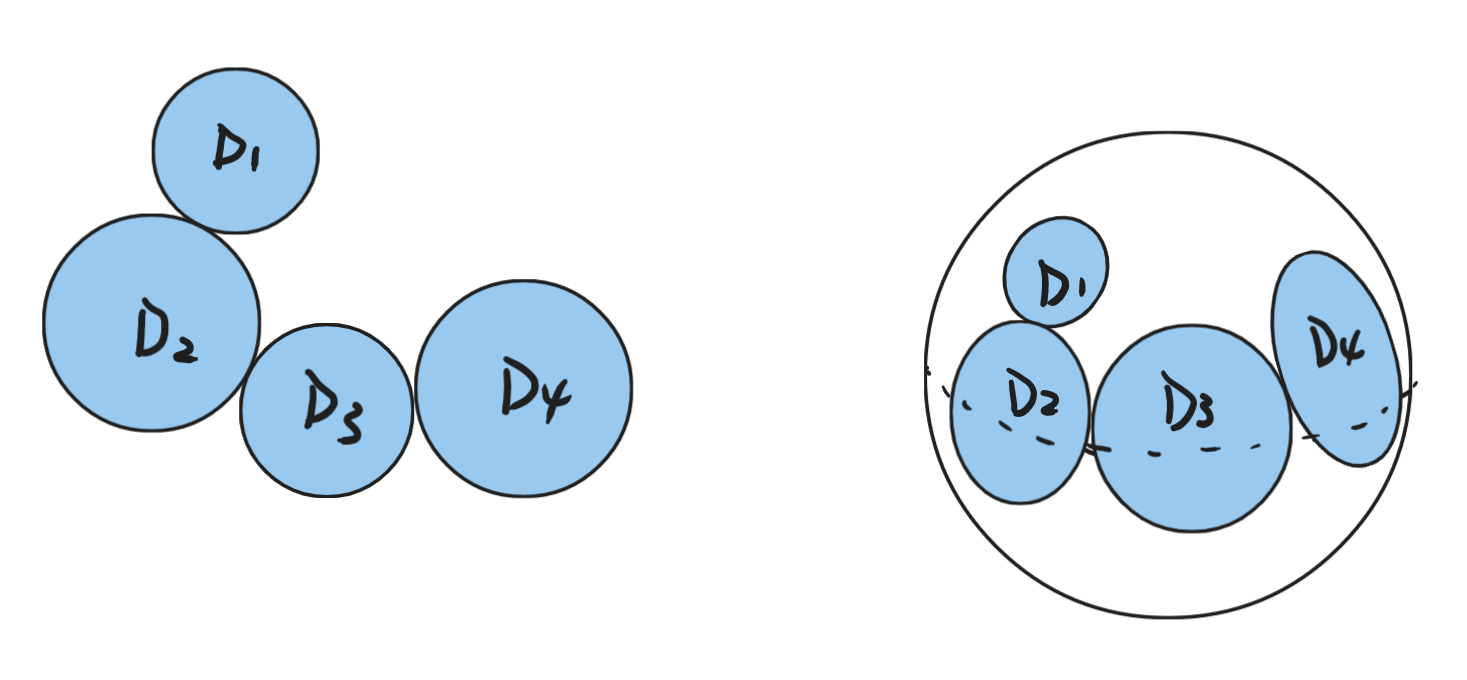
\includegraphics[width=\textwidth]{figures/kissingcaps.png}
\caption{From kissing disks to kissing caps}
\label{fig:kissing-caps}
\end{subfigure}
\caption{Kissing disks and caps}
\label{fig:kissing-disks-caps}
\end{figure}

The analogue of a disk on the sphere is a cap, which is given by the intersection of a half-space with the sphere, the boundary of which is a circle. We use stereographic projection to map the kissing disk embedding of the graph on the plane to a kissing cap embedding on the sphere. In further sections, we will show that we could always find a mapping that sends the centroid (center of gravity) of the centers of the caps to the center of the sphere.

\begin{theorem}
Let $G$ be a planar graph on $n$ nodes of degree at most $\Delta$, then the Fiedler value of $G$ is at most $\frac{16\Delta}{n}$
\end{theorem}

\begin{proof}
By theorem~\ref{Koebe-Andreev-Thurston} and theorem~\ref{th:sum_is_origin}, there is a representation of $G$ by kissing caps on the unit sphere so that the centroid of the centers of the caps is the center of the sphere. We let the center of the sphere be at the origin, and let $\vv_1,...,\vv_n$ be the centers of these caps, so that $\sum_{i=1}^{n}\vv_i=0$. As these vectors are on the unit sphere, $\|\vv_i\|=1$ for all $i$.

\begin{figure}[h]
\centering
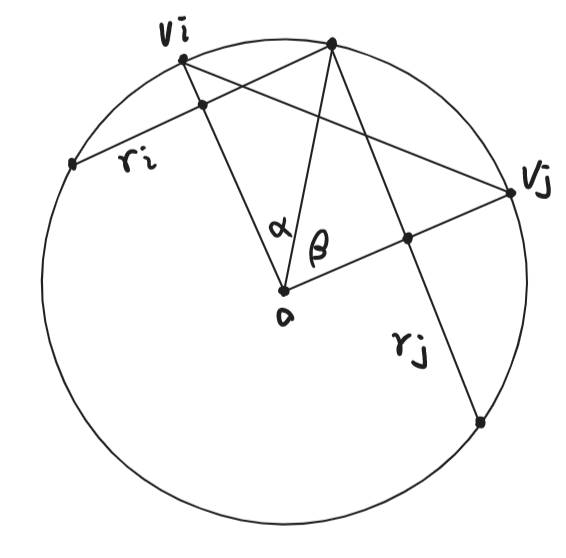
\includegraphics[width=0.3\textwidth]{figures/pmjh.png}
\label{fig:pmjh}
\caption{}
\end{figure}

 Let $r_1, ..., r_n$ be the radii of the caps, then the edge from $\vv_i$ to $\vv_j$ will have a squared length of at most $(r_i+r_j)^2 \leq 4(r_i^2 + r_j^2)$. We can prove it using elementary Euclidean geometry.
Let $r_1, ..., r_n$ be the radii of (the base of) the caps, and consider the length of $\vv_i$ to $\vv_j$ 
$\|\vv_i - \vv_j\| = 2\sin(\frac{\alpha+\beta}{2})$ \\
$r_i = \sin\alpha$, 
$r_j = \sin\beta$ \\
Let $u = \frac{\alpha +\beta}{2}, v = \frac{\alpha-\beta}{2}$, 
Consider 
\begin{align*}
\frac{r_i+r_j}{\|\vv_i - \vv_j\|}= &\frac{\sin\alpha + \sin\beta}{2\sin{\frac{\alpha+\beta}{2}}}= \frac{\sin(u+v)+sin(u-v)}{2\sin u} \\
 =&\frac{2\sin u \cos v}{2\sin u} = \cos v
\end{align*}
Since $v=\frac{\alpha-\beta}{2}$, $v$ satisfies $-\frac{\pi}{4} \leq u \leq \frac{\pi}{4}$, where $ \frac{\sqrt{2}}{2} \leq \cos v \leq 1$ always holds, and $\|\vv_i - \vv_j\| \leq \sqrt{2}(r_i + r_j)$

Consider all caps together, we have 
$$
\sum_{(i,j)\in E}\|\vv_i -\vv_j\|^2 \leq \sum_{(i,j)\in E} 2(r_i^2+r_j^2)\leq \sum_{(i,j)\in E} 4(r_i+r_j)^2 \leq 4\Delta\sum_{i=1}^{n} r_i^2
$$
as $\Delta$ is the max degree in the graph.

Since kissing caps do not overlap, the sum of the surface area of all caps is bounded by the surface area of the sphere, that is
$$
\sum_{i=1}^{n} \pi r_i^2 \leq 4\pi 
$$
therefore
$$
\sum_{(i,j)\in E}\|\vv_i -\vv_j\|^2  \leq 16\Delta
$$
Since we know that $\|\vv_i\|=1$ for all $i$, we have  $\sum_{i=1}^{n}\|\vv_i\|^2=n$, and hence
$$
\frac{\sum_{(i,j)\in E}\|\vv_i -\vv_j\|^2}{\sum_{i=1}^{n}\|\vv_i\|^2}  \leq \frac{16\Delta}{n}
$$
We then could apply theorem~\ref{embedding_lemma} (Embedding Lemma) to find that the Fiedler value of $G$ is at most $\frac{16\Delta}{n}$
\end{proof}

Since we retrieve the upper bound of the Fiedler value of $G$ to be $O(1/n)$, we could apply theorem~\ref{mihail} to get the upper bound of the ratio of the Fiedler cut to be $O(\sqrt{1/n})$. Then, according to Lemma~\ref{A1_lemma}, one can iterate Fiedler cuts to find a bisector of size $O(\sqrt{n})$.






% \begin{figure}
% \centering
% 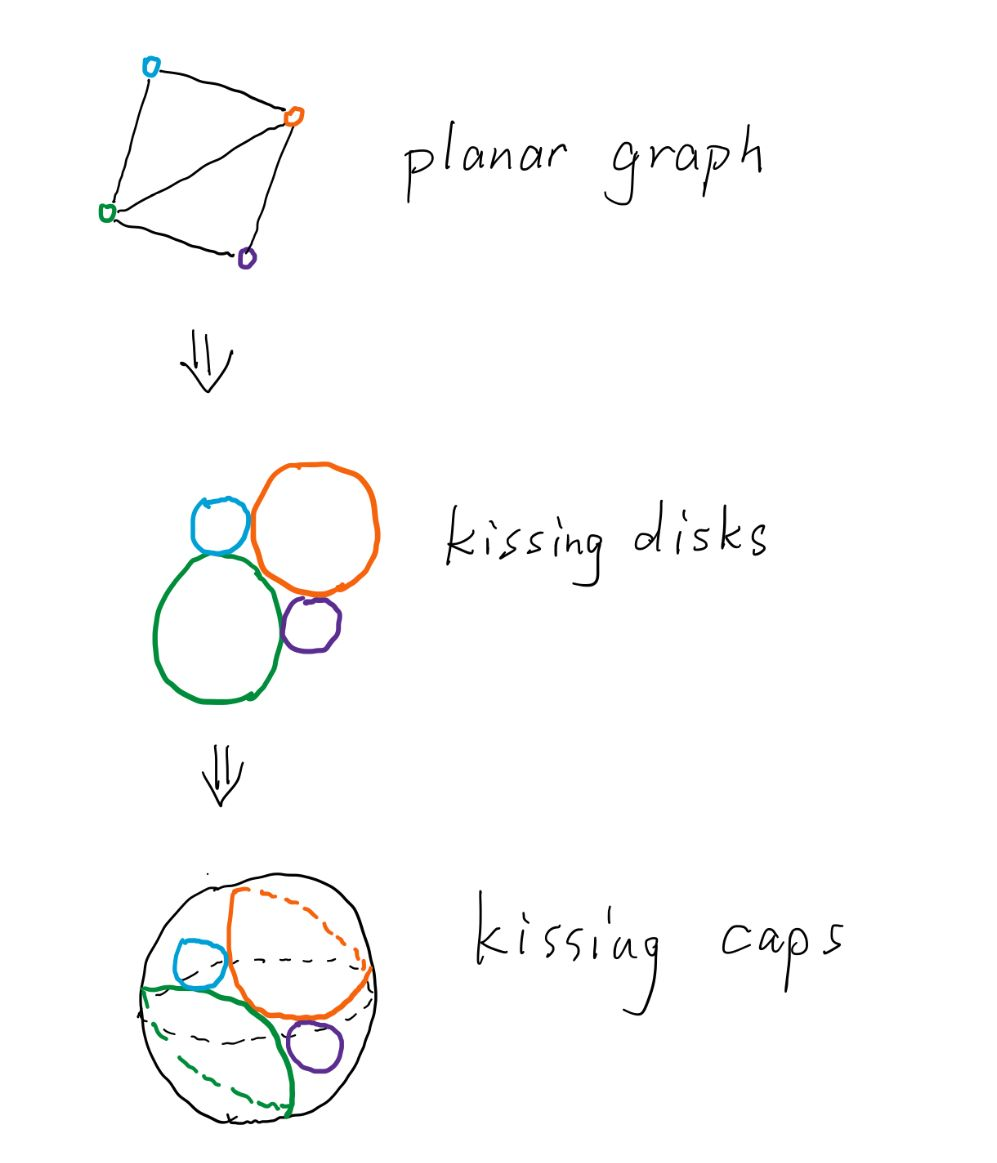
\includegraphics[width=0.5\textwidth]{figures/kissingcaps.jpg}
% \caption{The mapping from planar graphs to kissing disks and kissing caps}
% \label{fig:kissingcap}
% \end{figure}

% \begin{figure}
% \centering
% 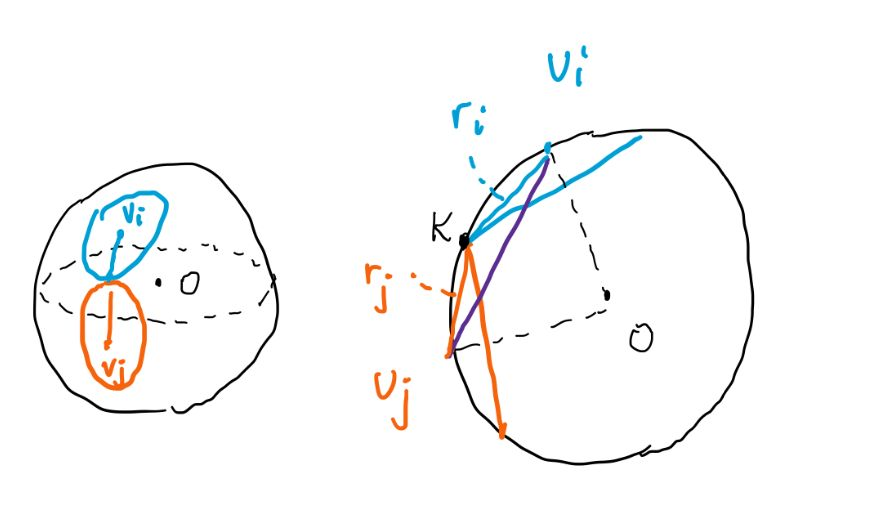
\includegraphics[width=0.5\textwidth]{figures/caps.jpg}
% \caption{The distance between the centers of two kissing caps}
% \label{fig:kissingcap}
% \end{figure}
